\documentclass[11pt]{article}
\usepackage[utf8]{inputenc}
\usepackage[T1]{fontenc}
\usepackage[margin=1in]{geometry}
\usepackage{amsmath}
\usepackage{booktabs}
\usepackage{graphicx}
\usepackage{hyperref}
\usepackage{natbib}
\usepackage{xcolor}
\usepackage{listings}
\usepackage{lmodern}
\usepackage{microtype}

\lstset{
  basicstyle=\ttfamily\small,
  columns=fullflexible,
  breaklines=true,
  frame=single,
  backgroundcolor=\color{black!3},
  literate={×}{{$\times$}}1
}

\title{tokentax: Measuring the Tokenizer Cost Penalty\\ Across 203 Languages}
\author{Shreyas K Chandrahas}
\date{}

\begin{document}
\maketitle

\begin{abstract}
The same sentence costs 1$\times$ tokens in English but roughly 9--11$\times$
in Shan, Santali, or Odia under current LLM tokenizers, because tokenizer
vocabularies are trained on English-heavy corpora. \citet{petrov2023} and
\citet{ahia2023} established this ``token tax'' for 2023-era tokenizers, but
no maintained, versioned resource reports current numbers for the tokenizers
actually in production use today. We present \texttt{tokentax}, a
measurement suite, versioned results dataset, and library that computes the
token premium, and its 95\% confidence interval via \texttt{evalci}
\citep{chandrahas2026evalci}, for 8 tokenizers (GPT-4o, GPT-4, GPT-2, Llama
3, Qwen2.5, DeepSeek-V3, Mistral, Gemma-2) across all 203 non-English
FLORES-200 languages \citep{nllbteam2022}. The pipeline reproduces
\citeauthor{petrov2023}'s published GPT-2/GPT-4 premium ratios within 1.1\%
relative error on five languages, a direct validation against prior work
rather than only internal self-consistency. Across the seven
currently-deployed tokenizers (excluding the 2019 GPT-2 vocabulary, which we
retain only as a historical anchor), the mean premium is 2.74$\times$ and
per-tokenizer means range from 2.13$\times$ (Gemma-2) to 3.16$\times$
(Mistral). Vocabulary size predicts the premium better than release year
does (Spearman $\rho=-0.91$ vs.\ $-0.76$), and Mistral -- a 2024 tokenizer
with the smallest vocabulary in our set -- carries a higher premium than
either 2024 tokenizer with a 200k+ vocabulary, so the improvement over time
is better read as a vocabulary-size effect than a release-date effect. A
domain-robustness check for the 30 highest-premium languages finds the
premium replicates closely on mixed-domain OPUS-100 text (median signed
difference $-1.7$\%) but runs systematically \emph{lower} on a
Bible-translation corpus (median $-17$\%, and lower in all 112 comparisons),
a register effect we report as a directional finding rather than as noise. 9
of those 30 languages have no modern, ungated parallel corpus on Hugging
Face for a second domain at all -- a scarcity that is itself part of the
token-tax story.
\texttt{tokentax} is available at \url{https://pypi.org/project/tokentax/}
(source: \url{https://github.com/Shreyaskc/token-tax}), with the full
results dataset and an interactive explorer at
\url{https://huggingface.co/datasets/shreyaskc/tokentax-results-v1} and
\url{https://huggingface.co/spaces/shreyaskc/tokentax-explorer}.
\end{abstract}

\section{Introduction}

Token-based API pricing and fixed context windows mean tokenizer
inefficiency is a real economic and capability penalty, not a cosmetic one.
If a language costs $k\times$ as many tokens as English for the same
content, its speakers pay $k\times$ as much per query, retain $1/k$ as many
effective few-shot examples in a fixed context window, and hit context
truncation $k\times$ sooner. \citet{petrov2023} first quantified this
systematically, finding tokenization-length disparities of up to 15$\times$
across languages for tokenizers available in 2023; \citet{ahia2023}
independently showed that OpenAI's commercial API pricing, applied uniformly
per token, overcharges speakers of many supported languages for equivalent
utility. \citet{rust2021} showed the same underlying disparity degrades
downstream monolingual task performance, not just cost.

These are foundational results, but the tokenizers they measured are no
longer the ones in production use. GPT-2's tokenizer (2019) and cl100k\_base
(2022, GPT-3.5/GPT-4) have both been superseded by larger, more
multilingual-aware vocabularies -- OpenAI's o200k\_base (GPT-4o), and
open-weight vocabularies from Meta, Alibaba, DeepSeek, Mistral, and Google.
Whether the token tax has actually improved with these newer vocabularies,
and by how much, is a question every multilingual-fairness paper since 2023
has had to re-derive ad hoc, because no maintained, versioned, statistically
rigorous resource reports current numbers. This is precisely the gap a
living benchmark should fill: the numbers change with every tokenizer
release, which argues for a re-runnable measurement suite and a versioned
dataset over a one-off paper.

We present \texttt{tokentax}: (1) a small Python library that computes the
token premium, bytes/characters-per-token, and effective context-window
shrinkage for any tokenizer against any parallel corpus, with confidence
intervals via \texttt{evalci} \citep{chandrahas2026evalci}; (2) a full sweep
of 8 current tokenizers against all 203 non-English FLORES-200 languages,
validated by reproducing \citeauthor{petrov2023}'s published numbers; (3) a
domain-robustness check against a second corpus for the 30 most heavily
taxed languages; and (4) a versioned results dataset and interactive
explorer, so the resource stays current as new tokenizers ship.

\section{Related Work}

\citet{petrov2023} is the direct precedent for this work: a systematic study
of tokenization-length disparity across languages for GPT-2, GPT-3, GPT-4,
and several open tokenizers of the time, using FLORES-200 as the parallel
corpus -- the same choice we make, for the same reason (Section~\ref{sec:methods}).
\citet{ahia2023} took the complementary economic angle, translating token
counts into actual API dollar costs and utility-per-dollar across 22
languages, and is the direct precedent for our cost-analysis framing
(Section~\ref{sec:cost}). \citet{rust2021} showed that a designated
monolingual tokenizer, not just pretraining data volume, materially affects
downstream task performance -- the capability-side consequence of the same
disparity we measure on the cost side. \citet{nllbteam2022} introduced
FLORES-200, the parallel-sentence corpus this entire line of work, including
ours, depends on.

\texttt{tokentax}'s contribution relative to this line of work is not a new
finding about \emph{why} the disparity exists -- that question is settled --
but a maintained instrument for \emph{how much} it currently is, built to be
re-run as tokenizers change, with every reported number carrying a
confidence interval rather than a bare point estimate, and with an explicit
domain-robustness check rather than a single-corpus measurement.

\section{The \texttt{tokentax} Suite}
\label{sec:methods}

\paragraph{Premium ratio.} For a tokenizer $T$ and an aligned sentence pair
$(s_{\mathrm{en}}, s_{\ell})$ expressing the same content in English and
language $\ell$, the per-sentence premium ratio is
$r_i = |T(s_\ell^{(i)})| / |T(s_{\mathrm{en}}^{(i)})|$, where $|T(\cdot)|$ is
token count. We compute this only on \emph{aligned parallel} sentences, never
independent monolingual corpora: only a shared-meaning pair makes ``language
$\ell$ costs $k\times$ as many tokens as English for the same content'' a
defensible claim, since monolingual corpora in different languages differ in
register, sentence length, and content independent of tokenization efficiency.

\paragraph{Estimand.} Every premium we report is the \emph{mean of
per-sentence ratios}, $\bar{r} = \frac{1}{n}\sum_i r_i$, which answers ``what
does a typical sentence cost?'' and admits a straightforward per-sentence
bootstrap. This is deliberately \emph{not} the ratio of corpus totals,
$\sum_i |T(s_\ell^{(i)})| \big/ \sum_i |T(s_{\mathrm{en}}^{(i)})|$, which
answers a different question (``what does the whole corpus cost?'') and
weights long sentences more heavily. The two differ: by Jensen's inequality
$\bar{r}$ is upward-biased relative to the ratio of totals, and across the
ten (language, tokenizer) pairs of Section~\ref{sec:validation} we measure
that bias at 0.9--1.7\%. This matters when comparing our numbers to prior
work, which generally reports the ratio of totals; see
Section~\ref{sec:validation}. Readers needing the other estimand can
recompute it from the released per-sentence data.

\paragraph{Corpus.} We use FLORES-200 devtest \citep{nllbteam2022}: 1{,}012
sentences, professionally translated in parallel into 200+ languages,
covering 203 languages with an English pairing in our sweep. FLORES-200 is
gated on Hugging Face (a free, instant license click, not a manual review).

\paragraph{Tokenizers.} We study 8 tokenizers, loaded via \texttt{tiktoken}
for OpenAI vocabularies and Hugging Face \texttt{transformers}
\citep{wolf2020transformers} for every open-weight one: OpenAI's
o200k\_base (GPT-4o) and cl100k\_base (GPT-4), and the legacy GPT-2
vocabulary (kept only for the validation in Section~\ref{sec:validation});
Meta's Llama 3; Alibaba's Qwen2.5; DeepSeek-V3; Mistral (v0.3); and
Google's Gemma-2. Two deviations
from the obvious choice, both discovered by actually running the pipeline
rather than assumed in advance: \texttt{meta-llama/Meta-Llama-3-8B} requires
Meta's manual license approval rather than an instant click-through, so our
Llama 3 tokenizer resolves to the widely-used, ungated
\texttt{NousResearch/Meta-Llama-3-8B} mirror of the same vocabulary (we have
not independently verified byte-for-byte equivalence against the gated
original; see Limitations); and Mistral's tokenizer turned out not to be
gated at all once tested, only
missing a \texttt{protobuf} runtime dependency. Anthropic's Claude is
excluded: it has no downloadable tokenizer artifact, only a token-counting
API endpoint, which would require every user reproducing this dataset to
hold an API key. Gemma-2's SentencePiece vocabulary is also the closest
available open proxy for Gemini's tokenizer, which likewise has no public
artifact; we report it only under the Gemma-2 name and do not present it as
a Gemini measurement.

GPT-2 is included as a \emph{historical anchor} for the trend analysis
(Section~\ref{sec:trend}) and for the validation in
Section~\ref{sec:validation}; it is not a currently-deployed tokenizer. We
therefore report aggregate statistics over the seven current tokenizers
separately from the full set of eight wherever the distinction changes the
number, and say which basis is in use each time.

Table~\ref{tab:tokenizers} lists vocabulary sizes, which
Section~\ref{sec:trend} uses to separate vocabulary-size effects from
release-date effects.

\begin{table}[htbp]
\centering
\small
\begin{tabular}{llrr}
\toprule
Tokenizer & Family & Vocab.\ size & Mean premium \\
\midrule
Mistral (v0.3) & Mistral     & 32{,}768  & 3.16$\times$ \\
GPT-2$^\dagger$ & OpenAI     & 50{,}257  & 4.48$\times$ \\
GPT-4 (cl100k\_base) & OpenAI & 100{,}277 & 3.42$\times$ \\
Llama 3        & Meta        & 128{,}256 & 3.04$\times$ \\
DeepSeek-V3    & DeepSeek    & 128{,}815 & 2.52$\times$ \\
Qwen2.5        & Alibaba     & 151{,}665 & 2.79$\times$ \\
GPT-4o (o200k\_base) & OpenAI & 200{,}019 & 2.15$\times$ \\
Gemma-2        & Google      & 256{,}000 & 2.13$\times$ \\
\bottomrule
\end{tabular}
\caption{Tokenizers studied, ordered by vocabulary size, with mean premium
over 203 non-English FLORES-200 languages. $^\dagger$GPT-2 is a 2019
historical anchor, not a currently-deployed tokenizer, and is excluded from
``current tokenizer'' aggregates.}
\label{tab:tokenizers}
\end{table}

\paragraph{Confidence intervals.} Every reported premium ratio is a
percentile bootstrap 95\% confidence interval over the 1{,}012 per-sentence
ratios, computed by \texttt{evalci.ci(method="bootstrap")}
\citep{chandrahas2026evalci} -- not reimplemented, per this project's
cross-artifact reuse policy.

\section{Validation Against Prior Work}
\label{sec:validation}

Rather than validate only against our own pipeline's internal consistency,
we reproduce \citeauthor{petrov2023}'s own published per-language token
totals over FLORES-200 devtest for GPT-2 and GPT-4's cl100k\_base, for five
languages spanning a range of scripts and premium magnitudes.\footnote{Reference
values computed from \url{https://github.com/AleksandarPetrov/tokenization-fairness},
the paper's own released data -- inferred from how that data is organized,
not confirmed against their paper text; the close agreement below is
evidence the inference is right.} Table~\ref{tab:validation} shows agreement
within 1.1\% relative error for every (language, tokenizer) pair -- well
inside the 2\% target we set before running it, and consistent with the
small differences expected from FLORES-200 dataset revisions since 2023.

One caveat deserves emphasis, because it is easy to overstate what this
table shows. To compare like with like, the reproduction column uses the
\emph{ratio of corpus totals}, matching how \citeauthor{petrov2023}'s
released data is organized -- not the mean-of-per-sentence-ratios estimand
used for every other number in this paper (Section~\ref{sec:methods}). What
Table~\ref{tab:validation} establishes is therefore that our
\emph{tokenization and corpus handling} agree with prior work to within
1.1\%; it does not independently validate the mean-of-ratios estimator,
which by construction runs 0.9--1.7\% higher on these same pairs. Both
quantities are computable from the released per-sentence data, and we report
which is which rather than blurring them into a single ``validated''
number.

\begin{table}[htbp]
\centering
\small
\begin{tabular}{lrrrr}
\toprule
Language & Tokenizer & Published & Reproduced$^\ast$ & Rel.\ error \\
\midrule
Amharic         & GPT-2 & 7.787  & 7.702  & 1.1\% \\
Amharic         & GPT-4 & 7.678  & 7.593  & 1.1\% \\
Tamil           & GPT-2 & 15.582 & 15.537 & 0.3\% \\
Tamil           & GPT-4 & 7.651  & 7.644  & 0.1\% \\
Burmese         & GPT-2 & 16.891 & 16.813 & 0.5\% \\
Burmese         & GPT-4 & 11.702 & 11.618 & 0.7\% \\
Hindi           & GPT-2 & 7.459  & 7.413  & 0.6\% \\
Hindi           & GPT-4 & 4.794  & 4.759  & 0.7\% \\
Standard Arabic & GPT-2 & 4.400  & 4.358  & 1.0\% \\
Standard Arabic & GPT-4 & 3.037  & 3.027  & 0.3\% \\
\bottomrule
\end{tabular}
\caption{Reproduction of \citet{petrov2023}'s published premium ratios.
Maximum relative error 1.1\% across 10 (language, tokenizer) pairs.
$^\ast$Computed as the ratio of corpus totals to match the reference data,
not the mean-of-per-sentence-ratios estimand used elsewhere in this paper;
the latter runs 0.9--1.7\% higher on these pairs.}
\label{tab:validation}
\end{table}

\section{Results}

\subsection{Distribution}

Across the seven current tokenizers $\times$ 203 languages (1{,}421 pairs),
the mean premium is 2.74$\times$, the median 2.08$\times$, and the range
spans 0.94$\times$ (Mandarin under DeepSeek-V3) to 15.33$\times$ (Shan under
GPT-4). Including the GPT-2 historical anchor raises the mean to
2.96$\times$ and extends the maximum to 19.12$\times$; we quote the
seven-tokenizer figures throughout unless stated otherwise, since GPT-2 is
not a tokenizer anyone deploys today.

The single sub-1$\times$ value is Mandarin Chinese under DeepSeek-V3
(0.94$\times$, 95\% CI [0.93, 0.95], excluding 1) -- a genuine exception
rather than noise, plausibly because a vocabulary trained with substantial
Chinese-language data can represent common multi-character sequences more
compactly per token than the corresponding English byte-pair merges do.
Notably, under current tokenizers the three lowest-premium languages are all
Chinese variants (Simplified 1.30$\times$, Cantonese 1.40$\times$,
Traditional 1.43$\times$), displacing the Latin-script European languages
that occupy those positions when GPT-2 is averaged in -- a concrete instance
of newer vocabularies redistributing the tax rather than uniformly lowering
it.

\subsection{Which languages are taxed the most}

Figure~\ref{fig:top-languages} shows the 15 languages with the highest mean
premium across the seven current tokenizers. All 11 languages above
6.5$\times$ are written in non-Latin scripts: Shan (Myanmar script), Santali
(Ol Chiki), Odia, Dzongkha and Tibetan (Tibetan script), Tamasheq and
Tamazight (Tifinagh), Lao, Burmese, Khmer, and Malayalam. At the opposite
end, the 10 lowest-premium languages (1.30--1.51$\times$) are Latin-script
European languages plus Indonesian and the three Chinese variants.

We deliberately stop at describing this as a script-level pattern. It is
tempting to explain it by how much text in each script appears in tokenizer
pretraining corpora, and that is very likely the mechanism
\citep{petrov2023,rust2021}; but we measure tokenizer output, not training
data, and the pretraining mixtures for six of our eight tokenizers are not
public. Establishing the mechanism would require corpus-composition data we
do not have, so we report the association and leave the causal claim to work
that can measure the input side directly.

\begin{figure}[htbp]
  \centering
  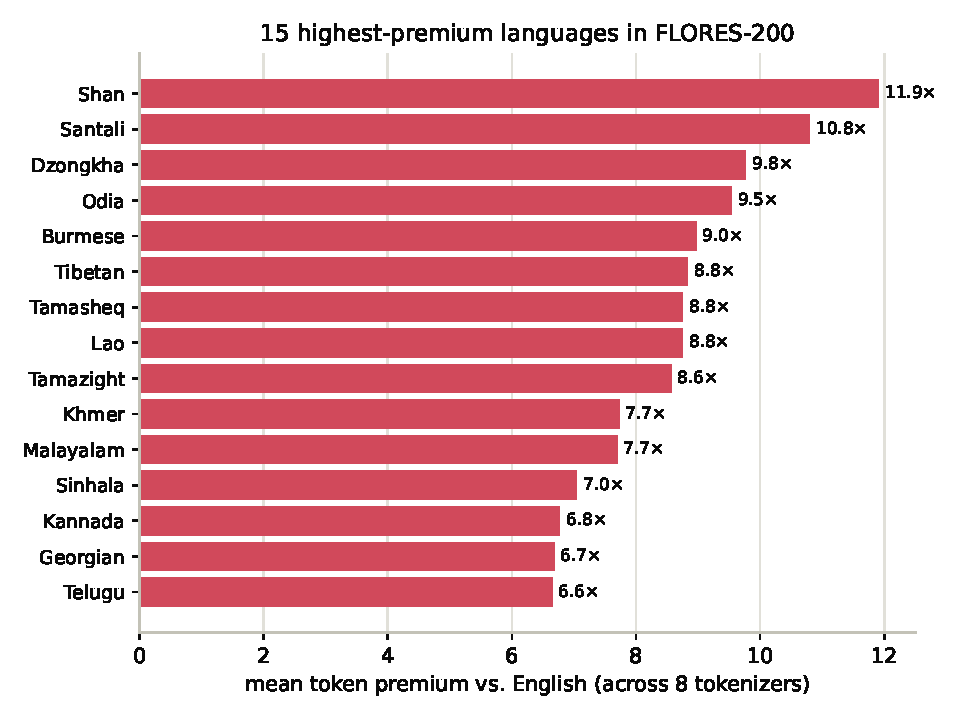
\includegraphics[width=0.85\textwidth]{figures/top_languages.pdf}
  \caption{15 languages with the highest mean token premium vs.\ English,
  averaged across the seven current tokenizers (GPT-2 excluded).}
  \label{fig:top-languages}
\end{figure}

\subsection{Vocabulary size, not release year}
\label{sec:trend}

Figure~\ref{fig:tokenizer-trend} orders the 8 tokenizers by mean premium.
All six 2024 tokenizers sit below GPT-4's 2022 cl100k\_base (3.42$\times$)
and GPT-2's 2019 vocabulary (4.48$\times$), and four of them (Gemma-2,
GPT-4o, DeepSeek-V3, Qwen2.5) come in at $\leq$2.8$\times$. That invites the
summary ``newer tokenizers are fairer.'' The summary is too coarse, and the
vocabulary sizes in Table~\ref{tab:tokenizers} show why.

Vocabulary size is the better predictor. Across the 8 tokenizers, mean
premium correlates with vocabulary size at Spearman $\rho = -0.91$
($p = 0.002$) but with release year at only $\rho = -0.76$ ($p = 0.027$);
Figure~\ref{fig:vocab} plots the former. The decisive case is Mistral: a
2024 tokenizer with the smallest vocabulary in our set (32{,}768) and a mean
premium of 3.16$\times$ -- barely better than the two-year-older GPT-4
vocabulary (3.42$\times$), and roughly 50\% worse than the two 2024
tokenizers with 200k+ vocabularies (2.13--2.15$\times$). Being recent buys a
language little if the vocabulary is small.

Two caveats keep this from being a clean causal claim. First, vocabulary
size is itself correlated with how much multilingual data went into training
the vocabulary, and we cannot separate the two from tokenizer artifacts
alone. Second, both pre-2024 baselines (GPT-2, GPT-4) come from a single
vendor, so ``older'' and ``OpenAI'' are partly confounded in the temporal
comparison -- though notably OpenAI's own o200k\_base is among the lowest-premium
vocabularies we measured, which cuts against reading the trend as a
vendor effect.

\begin{figure}[htbp]
  \centering
  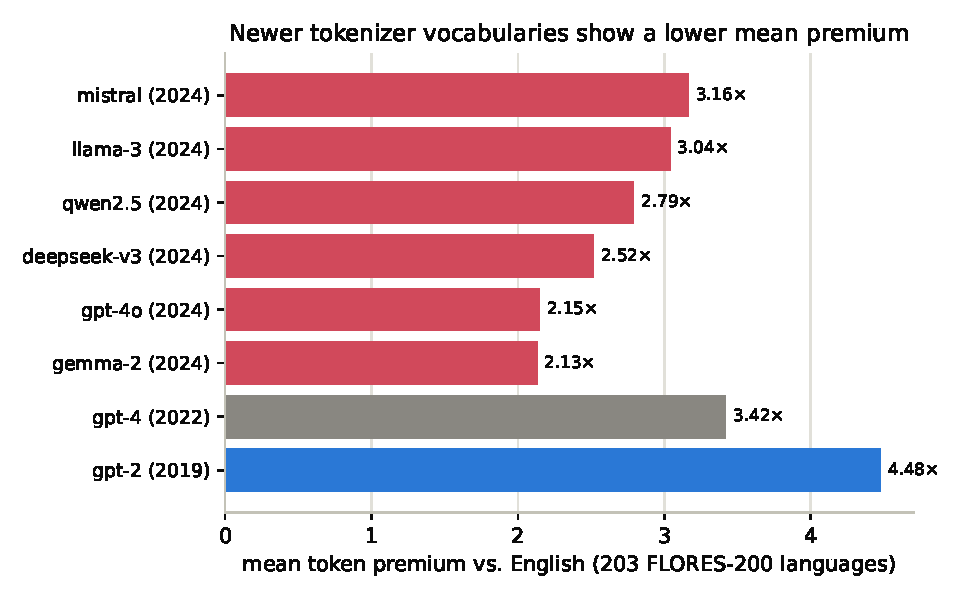
\includegraphics[width=0.85\textwidth]{figures/tokenizer_trend.pdf}
  \caption{Mean token premium by tokenizer, colored by approximate release
  era of the associated model family (blue: 2019, gray: 2022, red: 2024).
  Release years reflect the model family's public release, not necessarily
  the exact date the tokenizer vocabulary itself was frozen.}
  \label{fig:tokenizer-trend}
\end{figure}

\begin{figure}[htbp]
  \centering
  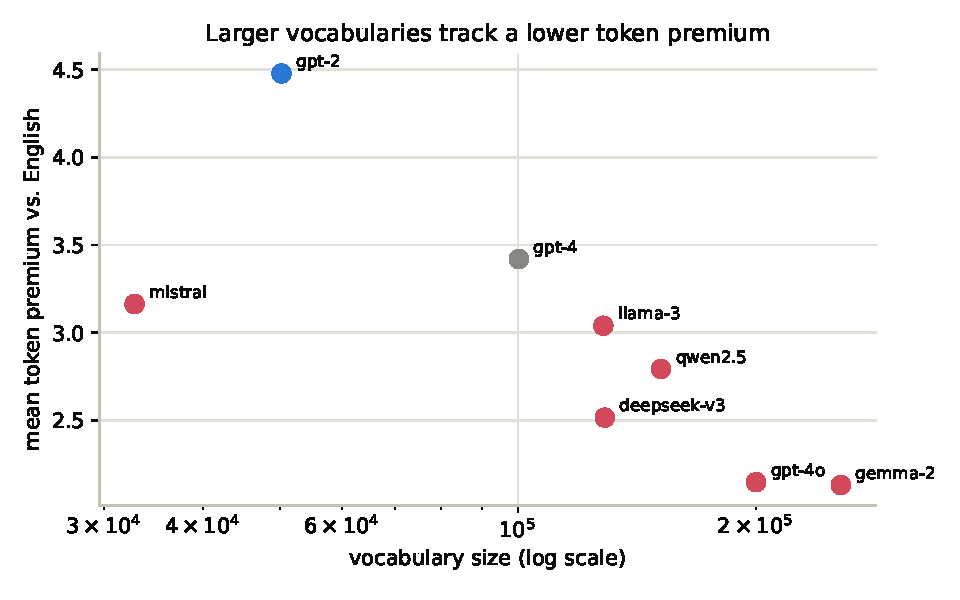
\includegraphics[width=0.8\textwidth]{figures/vocab_vs_premium.pdf}
  \caption{Mean token premium against vocabulary size (log scale), colored
  by release era as in Figure~\ref{fig:tokenizer-trend}. Mistral (2024,
  32{,}768 tokens) sits well above the 2024 tokenizers with larger
  vocabularies, and GPT-2 is both the oldest and among the smallest --
  vocabulary size tracks the premium more closely than release year does.}
  \label{fig:vocab}
\end{figure}

\subsection{Domain robustness}
\label{sec:domain-robustness}

FLORES-200 is encyclopedic/news-register text; a premium ratio that only
replicates on that one register is a weaker claim than one that holds
across registers. For the 30 languages with the highest mean FLORES premium,
we additionally measured the premium on a second corpus where one exists:
mixed-domain OPUS-100 text \citep{zhang2020opus100} and/or the eBible
Corpus \citep{akerman2023ebible} (religious register), each with its own
aligned English pairing (not FLORES's).

Of these 30 languages, 21 have at least one second-domain corpus available;
the other 9 -- Shan, Santali, Tibetan, Tamasheq, Tamazight, Lao, Tigrinya,
Manipuri, and Kabiy\`{e} -- have no modern, ungated, actively-maintained
parallel corpus on Hugging Face for a second domain at all. We report this
gap explicitly rather than silently narrowing the check to the languages
that happen to have data: the languages with the highest token tax are, by
this evidence, also among those with the least available parallel data to
independently corroborate it, which is itself a relevant fact for
multilingual-NLP resource allocation.

Across the 264 (language, tokenizer, domain) comparisons where a second
corpus exists, the median \emph{absolute} relative difference from the
FLORES estimate is 14\% (mean 17\%). Reporting only that figure would be
misleading, because the two domains behave very differently once the sign is
retained.

On OPUS-100 the difference is genuinely symmetric noise: median signed
difference $-1.7$\%, with 57\% of comparisons falling below the FLORES
estimate -- about what chance would give. On the Bible corpus it is not
noise at all. The median signed difference is $-17.2$\%, and the domain
premium is lower than the FLORES premium in \emph{all 112} comparisons.
A sign test against the null of symmetric divergence gives $p < 10^{-30}$;
this is a systematic register effect, not sampling variation.

We therefore read the Bible-corpus result as a finding rather than a
caveat: on religious-register parallel text, the token premium is
consistently around a sixth lower than on FLORES's encyclopedic register.
The plausible mechanism is that these translations use a smaller, more
repetitive, more standardized vocabulary than news and encyclopedia prose,
which favors any subword tokenizer in the non-English language; but we have
not tested that, and it is equally consistent with these particular
translations being older and more heavily edited than the FLORES sentences.
The practical implication for users of this dataset is that a premium ratio
is a property of a (tokenizer, language, register) triple, not of a
(tokenizer, language) pair, and quoting one should say which register it
came from.

Individual outliers remain worth flagging: Kannada on OPUS-100 diverges up
to 107\%, most likely a short, UI-string-heavy test split rather than a
general property of the language, and Uyghur and Sanskrit on the Bible
corpus diverge 44--72\%, beyond even that domain's systematic shift.

\subsection{Cost analysis}
\label{sec:cost}

Following \citet{ahia2023}'s framing, Table~\ref{tab:cost} converts premium
ratios into dollar terms: at the \$2.50-per-million-input-token figure for
GPT-4o in our released pricing table -- a placeholder snapshot explicitly
marked unverified against current provider pricing, not a confirmed
current price (see Limitations) -- the same 1-million-token quantity of
content costs \$2.50 in English but up to \$34.82 in Santali -- a
13.9$\times$ markup for identical meaning, before any consideration of the
additional latency and context-window cost of the extra tokens.

\begin{table}[htbp]
\centering
\small
\begin{tabular}{lrr}
\toprule
Language & Premium (GPT-4o) & Cost for content worth 1M English tokens \\
\midrule
Santali    & 13.93$\times$ & \$34.82 \\
Tamasheq   & 10.41$\times$ & \$26.04 \\
Tamazight  & 10.26$\times$ & \$25.65 \\
Dzongkha   & 9.22$\times$  & \$23.06 \\
Lao        & 8.38$\times$  & \$20.94 \\
Tibetan    & 8.23$\times$  & \$20.56 \\
Shan       & 8.10$\times$  & \$20.26 \\
Tigrinya   & 6.05$\times$  & \$15.13 \\
Amharic    & 5.85$\times$  & \$14.63 \\
Odia       & 5.05$\times$  & \$12.62 \\
\midrule
English (baseline) & 1.00$\times$ & \$2.50 \\
\bottomrule
\end{tabular}
\caption{Cost to process 1 million English-tokens' worth of equivalent
content, by language, at GPT-4o's input-token price in our released
pricing table. Pricing is an unverified placeholder snapshot, not a
confirmed current price; see Limitations.}
\label{tab:cost}
\end{table}

\section{Limitations}

The premium we report is a mean of per-sentence ratios, which is
upward-biased by roughly 1--2\% relative to the ratio-of-totals estimand
that prior work generally reports (Section~\ref{sec:methods}). Comparisons
against published figures should account for this; both quantities are
recoverable from the released per-sentence data.

The vocabulary-size finding (Section~\ref{sec:trend}) rests on 8 tokenizers,
which is a small sample for a correlation, and vocabulary size is not
randomly assigned -- it covaries with how much multilingual data the
vocabulary was trained on, which we cannot observe for six of the eight.
Both pre-2024 baselines are also OpenAI vocabularies, partly confounding
``older'' with vendor in the temporal comparison. We report the association
and the one case that discriminates between the two explanations (Mistral),
not a controlled result.

The domain-robustness check (Section~\ref{sec:domain-robustness}) covers 21
of the 30 highest-premium languages, not all 203, and the 9 uncovered
languages are systematically the most extreme cases rather than a random
sample -- so neither the OPUS-100 agreement nor the Bible-corpus offset
should be extrapolated to languages outside the 21 actually checked. All
three corpora consist of translated rather than natively-authored text,
which may introduce a shared translationese effect that a monolingual
comparison would not have; the Bible-corpus offset we report is a difference
between two translated registers, not between translated and natural text.

Pricing figures (Section~\ref{sec:cost}) are a static, manually-maintained
snapshot explicitly marked \texttt{verified: false} in the released pricing
table; the library warns on load until a maintainer confirms current
provider pricing, and dollar figures should be treated as illustrative of
magnitude, not as a citable current price. Claude is excluded from every
result in this paper for the reason given in Section~\ref{sec:methods}, not
because it is exempt from the phenomenon. The Llama 3 tokenizer is measured
via an ungated third-party mirror, not Meta's own gated repository. Gemma-2
is reported only as itself, not as a validated proxy for Gemini's
(unpublished) tokenizer. Finally, every number in this paper reflects
specific tokenizer commits, recorded in the released code
(Section~\ref{sec:availability}); the five Hugging Face-hosted tokenizers
were originally measured against their \texttt{main} branch rather than a
frozen commit, which we have since corrected by pinning the registry to the
exact commit \texttt{main} resolved to at that time (verified to reproduce
identical token counts). Tokenizer vocabularies are periodically updated by
their maintainers, and the versioned dataset, not this PDF, is the source
of truth for current numbers.

\section{Ethics Statement}

This work is a measurement, not a system: it does not collect, generate, or
redistribute personal data, and the released dataset contains only token
counts, premium ratios, and confidence intervals -- never the underlying
FLORES-200, OPUS-100, or Bible-corpus sentence text, which remain under
their original sources' own licenses. The motivating concern is fairness:
speakers of the languages in Table~\ref{tab:cost} and
Figure~\ref{fig:top-languages} pay materially more for equivalent access to
commercial language models, a disparity this paper aims to make legible and
citable rather than to newly create. We are not aware of a plausible
dual-use or harm pathway specific to this artifact; the intended use is
informing tokenizer design, pricing-policy discussion, and multilingual-NLP
methods sections that need a current, citable number.

\section{Availability}
\label{sec:availability}

\texttt{tokentax} is released under the MIT license (results dataset under
CC0) and available via \texttt{pip install tokentax}
(\url{https://pypi.org/project/tokentax/}). Source, the full sweep and
domain-robustness scripts, and tests are at
\url{https://github.com/Shreyaskc/token-tax}. The versioned results
dataset -- 1.64M raw per-sentence rows, the CI-backed summary table, and the
domain-robustness comparisons -- is at
\url{https://huggingface.co/datasets/shreyaskc/tokentax-results-v1}, and an
interactive heatmap and cost calculator at
\url{https://huggingface.co/spaces/shreyaskc/tokentax-explorer}. Continuous
integration runs the test suite across Python 3.9--3.12 on every push.

\section{Conclusion}

The token tax is not a 2023 finding that has since been fixed. Across the
seven currently-deployed tokenizers we measured, it persists at a mean of
2.74$\times$ and reaches 15$\times$ for the worst (language, tokenizer)
pair. Even the two lowest-premium 2024 vocabularies still charge Georgian,
Kannada, or Malayalam speakers roughly 2--4$\times$ English's rate for
identical content, and Qwen2.5 -- released the same year -- charges those
same three languages 5--7$\times$.

The more useful summary is not that tokenizers got better with time but
that they got better with vocabulary size: across our set, vocabulary size
predicts the premium substantially better than release year, and the 2024
tokenizer with the smallest vocabulary is barely an improvement on a
vocabulary two years its senior. That reframing matters for anyone choosing
a model for a non-English deployment, and it is actionable in a way that
``newer is fairer'' is not.

What will keep changing is the number itself. \texttt{tokentax} is built to
be re-run, not re-derived: the
measurement suite, the versioned dataset, and the explorer are designed so
that the next tokenizer release gets a new, citable number within days,
not another ad hoc re-implementation of \citeauthor{petrov2023}'s original
analysis.

\bibliographystyle{plainnat}
\bibliography{references}

\end{document}
